\section{Historical Context}

    \todo{Ever since the time of the earliest human civilizations, ...} \\
    \todo{Humans have been intrigued by the ... night sky.} \\
    \todo{Even before the invention of telescopes, with the naked eye alone...} \\
    \todo{Several bright objects could be distinguished from the rest of the night sky} \\
    \todo{Distinguish planets from stars, they exhibit relative motion ("planetes").} \\
    \todo{Ptolemai: Earth as center of the universe.} \\
    \todo{Copernicus: Sun as center of the Solar System.} \\
    \todo{Kepler: Kepler's laws, ellipsoid trajectories.} \\
    \todo{Newton: law of gravitation.} \\
    \todo{Discovery of planets in our solar system.} \\
    \todo{Discovery of exo-planets} \\
    \todo{Question: How do planets form?}
        
\section{Planet Formation}

    % The Interstellar Medium {{{
    \subsection{The Interstellar Medium}

        % What is the interstellar medium?
        The term \textit{interstellar medium} (ISM) is used to denote the matter and radiation that 
        can be found in the expanse of space between the stellar systems inside a galaxy. 
        As we will discuss further in the following sections, the ISM is widely considered to serve 
        as the birthplace of proto-planetary disks (PPDs), and subsequently, stars and planets. \\

        At first glance, it might not be easy to imagine how such giant objects like planets and 
        even stars can form in the ISM. After all, one might naively say that it consists of mostly
        nothing. From the point of view of a human living on Earth, the interstellar regions of
        outer space appear to be a near-perfect vacuum. \\

        Measurements of the the molcular particle number density in the ISM have been made in 
        previous studies by e.g. \cite{burton_2013}. Here, they showed that the number of particles 
        per unit volume can range from $\SI{1e16}{\meter^{-3}}$ all the way down to 
        $\SI{1e3}{\meter^{-3}}$. \\

        The exact value of the particle number density depends of course heavily on the precise 
        position in the ISM. Nonetheless, a comparison of the mere orders of magnitude involved 
        here demonstrates the huge difference in particle abundances in the ISM when compared to 
        Earth, where the number of gas molecules inside the atmosphere is approximately 
        $\SI{1e25}{\meter^{-3}}$.
        \footnote{Here we assume the validity of the ideal gas law, a sea-level pressure of 
                  $p=\SI{1}{\bar}$, and a temperature of $T=\SI{25}{\celsius}$.}
        \\

        The fact that giant astronomical objects like PPDs, stars, and planets can form from the 
        material found in the ISM, can be understood more easily if one brings to mind the
        absolutely enormous scales of both space and time that are involved here. \\

        Over time scales of (\todo{approx. how many years?}), the material in the ISM 
        will, under the effect of gravity, gather in giant interstellar clouds. Examples for such 
        clouds are given by e.g. \todo{(examples for clouds)}, measurements of which can be seen 
        visualized in \todo{(cite figures)}. \\

        \todo{Images of interstellar gas clouds, star-forming regions.} \\
        \todo{How big are they? How many light years across, approximately?} \\

        \vfill
\begin{figure}[h!]
    \centering
    \begin{minipage}{.5\linewidth}
        \centering
        \subfloat[Orion Nebula (Messier 42) \cite{orion_nebula_hubble_2006}]{
            \label{:a}
      	  	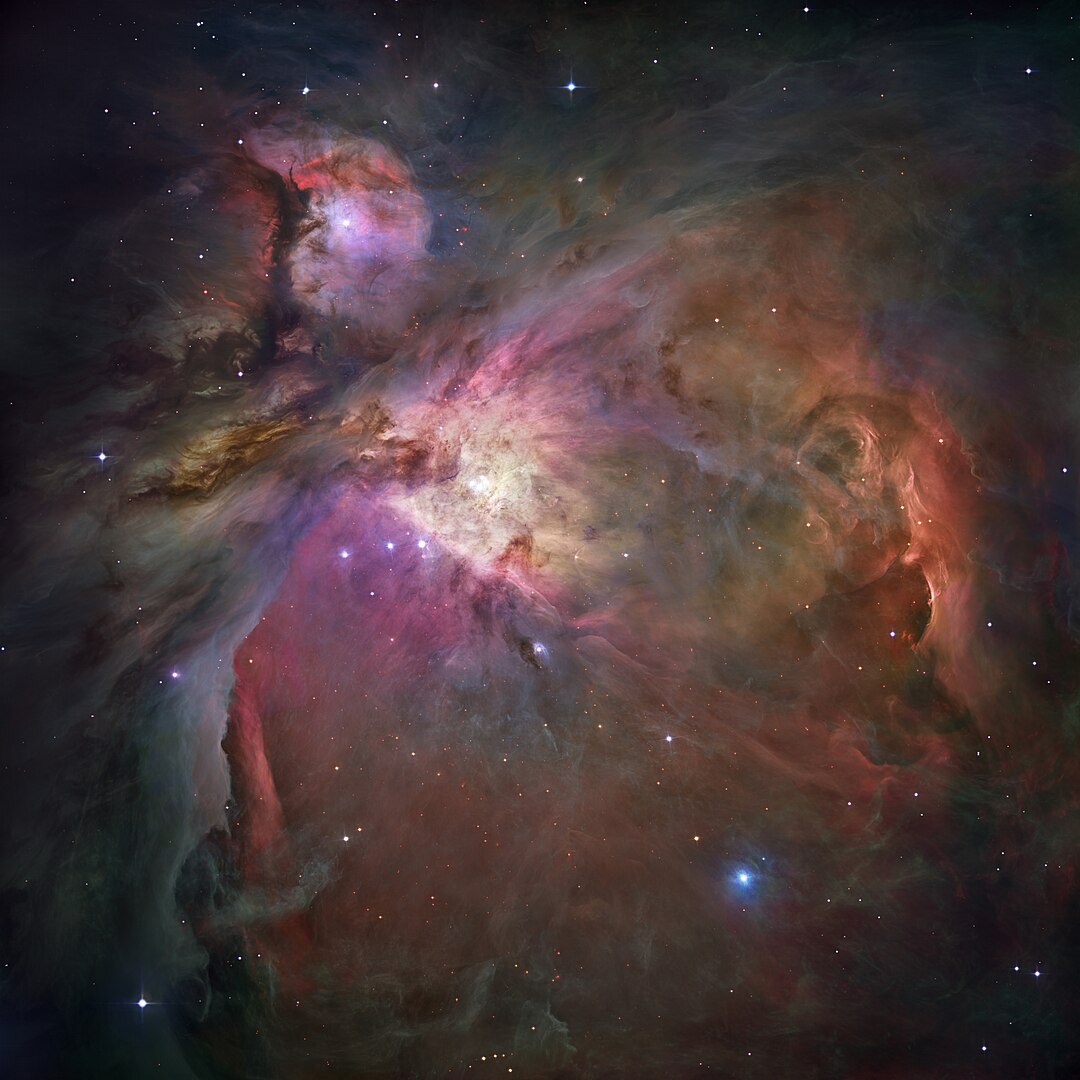
\includegraphics[width=0.85\linewidth]{Orion_Nebula_-_Hubble_2006_mosaic_1080px}
      	}
    \end{minipage}%
    \begin{minipage}{.5\linewidth}
        \centering
        \subfloat[Eagle Nebula (Messier 16) \cite{eagle_nebula_eso_2009}]{
            \label{:b}
            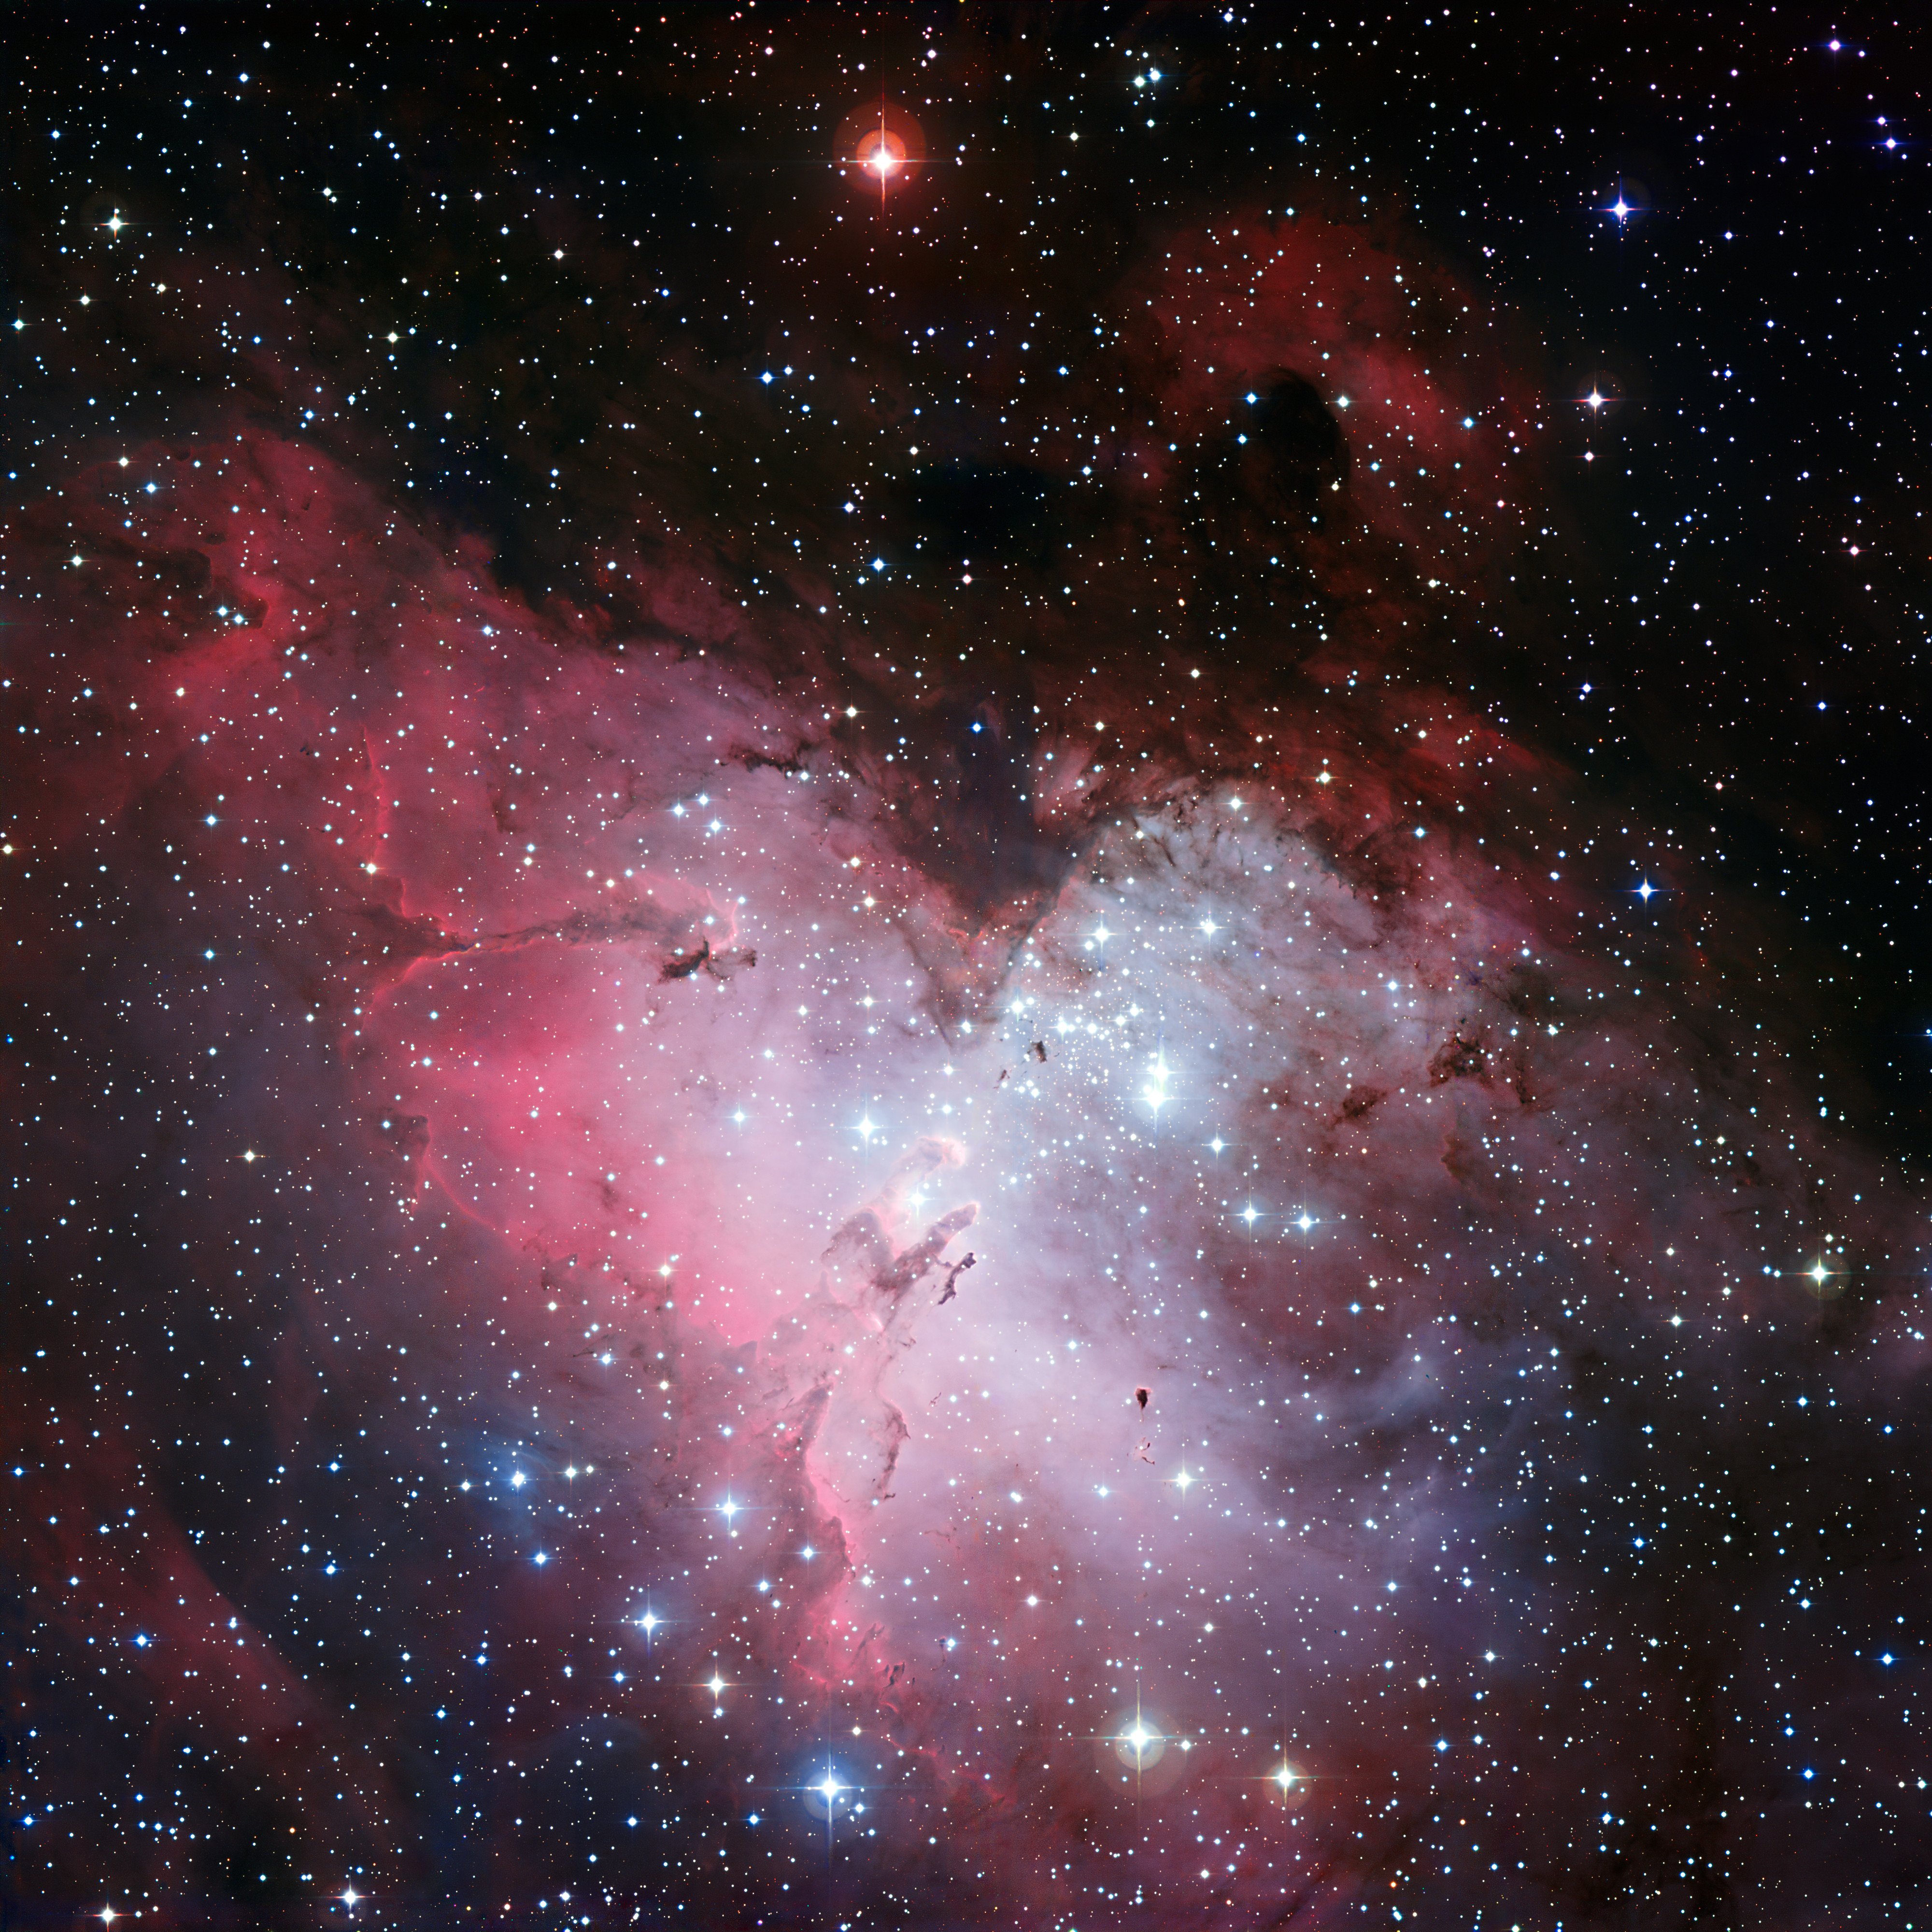
\includegraphics[width=0.85\linewidth]{eso0926a.jpg}
      	}
    \end{minipage}
    \caption{Examples of star-forming regions: (a) The Orion Nebula (b) The Eagle Nebula
        (Zoom in to see the famous \textit{Pillars of Creation} at the center of the image).
    }
    \label{fig:star_forming_regions}
\end{figure}


        The material making up these clouds can be classified into three main categories:
        \begin{enumerate}
            \item Molecular Gas: \\
                \todo{Mostly diatomic hydrogen $\text{H}_2$.} \\
                \todo{some helium, lithium, and trace amounts of heavier elements.}
            \item Ionized Gas: (Plasma) \\ 
                \todo{}
            \item Dust: \\
                \todo{Agglomerates of ...} \\
                \todo{held together (weakly) by ...} \\
                \todo{Shape: (fractal?)}
        \end{enumerate}

        Now that we've taken a brief look at the material make-up and particle density of the ISM, 
        let us turn our attention to the question of how PPDs, stars, and planets can be formed 
        from the aforementioned clouds of gas and dust.

    % }}}
    % The Nebular Hypothesis {{{ 
    \subsection{The Nebular Hypothesis}

        The \textit{nebular hypothesis} is a widely accepted model for explaining the formation and 
        evolution of not only our own Solar System, but the planetary systems around other stars as 
        well. 

        It was postulated independently by Immanuel Kant        % TODO cite
        and Pierre-Simon Laplace                                % TODO cite
        in 1755 and 1796, respectively. \\                      % TODO "independently" is that true?

        The hypothesis is built upon the idea that the formation of proto-planetary disks (and thus 
        solar systems) can be explained via the gravitational collapse of giant interstellar clouds 
        of gas and dust. (\todo: Examples for such star-forming regions, see above [cite]) \\
        \todo{(molecular clouds)}

        \todo{What is there at the beginning?}
        \begin{itemize}
            \item a giant cloud of (mostly) gas in the interstellar medium 
                  (as said before: mostly di-atomic hydrogen, and mono-atomic helium)
        \end{itemize}
        \todo{How big is such a cloud?}
        \begin{itemize}
            \item ...
        \end{itemize}
        \todo{What happens?}
        \begin{itemize}
            \item The cloud collapses under its own gravity. \todo{Cause?}
            \item The cloud posseses a total angular momentum. It is most likely $\neq 0$.
            \item Therefore, the cloud does not just simply collapse into a single point. 
                  (\todo{...})
            \item The cloud flattens into a disk.
            \item The majority of the mass present in the cloud gathers in the center.
            \item The rest of the mass flattens into a disk orbiting the star 
                  (later: solar system).
            \item In the center/core, density and temperature increase to a point that nuclear 
                  fusion becomes possible.
        \end{itemize}

        \todo{Result: PPD} \\
        \todo{Images of PPDs.}

    % }}}
    % The Road from Dust to Planet {{{ 
    \subsection{The Road from Dust to Planet}

        \todo{Evolution over many orders of magnitude.} \\
        \todo{Start with gas.}

        \todo{Then: dust particles}
        \begin{itemize}
            \item How do they form?
        \end{itemize}

        \todo{Then: dust agglomerates}
        \begin{itemize}
            \item They form via Coulomb and/or Van-der-Waals interactions
            \item Particles collide and, under the right circumstances, stick together.
            \item Larger and larger agglomerates form.
            \item They possess a fractal shape (dust bunnies).
        \end{itemize}
        \todo{Image of dust bunnies/fractals.}

        \todo{Then: pebbles} \\
        \todo{Then: planetesimals} \\
        \todo{Then: planetary cores (may start accreting gas)} \\
        \todo{Then: terrestrial planets} \\
        \todo{Then: gas giants (outer regions?)} \\

        \todo{Visualize particle coagulation.}

    % }}}

\section{Motivation for this Thesis}

    \todo{Why is planet formation relevant tous at all?} \\
    \todo{Why is dust coagulation relevant to planet formation?} \\
    \todo{How can one model dust coagulation?} \\
    \todo{What are the challenges involved in that model? (int. of Smol. eq.)} \\
    \todo{How does this thesis help with that?} 

\section{Structure \& Layout of this Thesis}

    \todo{What are the "parts" of this thesis?}
    \begin{enumerate}
        \item Disk model: disk, gas, \& dust.
        \item Coagulation \& Fragmentation: Smoluchowski equation, kernel, integration.
        \item Sampling: Probability distribution, results, stability \& accuracy.
    \end{enumerate}

\newpage
\section{Preliminary Notes on Axis Discretization}

    Throughout this thesis, we will deal with several physical quantities carrying values that 
    range across many orders of magnitude. Most notably, these are time, distance, and mass. \\

    As we will discuss later on, the differential equation(s) most relevant to this thesis only 
    possess analytical solutions in a very limited set of cases. Due to this fact, it will be
    necessary to make use of numerical integration techniques to obtain an approximate solution.
    As such, the axes for the above-mentioned (?) physical quantities will have to be discretized 
    in an appropriate manner. \\

    As an example, we will shortly demonstrate how one might do this for the mass axis $m$. The
    construction of a discrete axis for both time $t$ and space (i.e. radial distance $r$ from the
    central star) can then be done entirely analogously to what we will showcase here: \\

    The continuous range $m$ of particle masses present in the disk is partitioned into a set of 
    $\mathcal N_m\in\mathbb N$ intervals, which we will refer to as "bins" from this point onwards. 
    Each of these bins can be uniquely characterized by an index 
    $i\in[1,\mathcal N_m]\cap\mathbb N$, and assigned a corresponding mass value $m_i^\text{c}$, 
    which is situated at the \textit{center of the bin} (ergo the superfix "c").\\
    
    To derive an expression that can be used to calculate the mass values at these bin centers, 
    let us first define the mass values at the \textit{boundaries of the bin}. To do this,
    consider a collection of $\mathcal N_m+1$ appropriately spaced grid points $m_i^\text{b}$. 
    The first and last of these values, i.e. the lower and upper boundaries of the discrete mass 
    grid, shall be labeled $m_\text{min}$ and $m_\text{max}$, respectively. \\

    The spacing of the grid points of course depends heavily on the utilized scaling. In
    \cref{subsec:axis_discretization_with_linear_scale} and
    \cref{subsec:axis_discretization_with_logarithmic_scale}, we will go into more detail on how 
    exactly the values for $m_i^\text{b}$ and $m_i^\text{c}$ are to be defined when making use of 
    a linear and logarithmic scaling, respectively. \\
    % TODO Assure consistent usage of \text{b} and \text{c}.

    For the moment, a schematic represenation of the continuous mass axis and its discrete analogon
    can be seen visualized in \cref{fig:continuous_and_discrete_mass_axis} below.
    % TODO Display `Figure` instead of `fig`.

    \vfill

\begin{figure}[h!]
    \begin{center}
        \begin{tikzpicture}
            \def\N{5}      % This is the number of cells drawn (to the left of "..." separator).
            \def\M{6}      % This is the number of boundary arrows drawn (left of "...").
            \def\W{1.5}    % This is a cell's width.
            \def\H{\W}     % This is a cell's height.
            \def\L{\W/4}   % This is an arrow's length.
            \def\P{\W/8}   % This is the padding between arrow & cell.
            \def\R{\W/32}  % This is the padding between arrow & text.

            % Draw continuous mass axis.
            \draw [|-to](0, 2.5*\H) -- (\N*\W+4*\W, 2.5*\H);
            \draw [-](\W, 2.45*\H) -- (\W, 2.55*\H);
            \draw [-](\N*\W+3*\W, 2.45*\H) -- (\N*\W+3*\W, 2.55*\H);
            \node[] at (-2*\P, 2.5*\H) {$0$};
            \node[] at (\N*\W+4*\W+2*\P, 2.5*\H) {$m$};

            % Draw arrow from continuous to discretized mass axis.
            % \node[] at (\N*\W/2+1.5*\W, 2.25*\H) {$\Downarrow$};

            % Draw cells...
            % ...to the left of "..." separator.
            \foreach \x in {1, ..., \N} {
                \draw[draw=black] (\x*\W, 0) rectangle ++(\W, \H);
            }
            % ...to the right of "..." separator.
            \draw[draw=black] (\N*\W+2*\W, 0) rectangle ++(\W, \H);

            % Draw crosses...
            % ...to the left of "..." separator.
            \foreach \x in {1, ..., \N} {
                \draw (\x*\W+\W/2, \H/2) node {\tiny x};
            }
            % ...to the right of "..." separator.
            \draw (\N*\W+2.5*\W, \H/2) node {\tiny x};

            % Draw "..." separator.
            \node[] at (\N*\W+1.5*\W, \H/2) {...};

            % Draw arrows labeling cell boundaries.
            \foreach \x in {1, ..., \M} {
                \draw [-to](\x*\W, \H+\L+\P) -- (\x*\W, \H+\P);
                \node[] at (\x*\W, \H+\L+\P+\L+\R) {$m_\x^\text{b}$};
            }
            \draw [-to](\N*\W+2*\W, \H+\L+\P) -- (\N*\W+2*\W, \H+\P);
            \draw [-to](\N*\W+3*\W, \H+\L+\P) -- (\N*\W+3*\W, \H+\P);
            \node[] at (\N*\W+2*\W, \H+\L+\P+\L+\R) {$m_{\mathcal N_m}^\text{b}$};
            \node[] at (\N*\W+3*\W, \H+\L+\P+\L+\R) {$m_{\mathcal N_m+1}^\text{b}$};

            % Draw arrows labeling cell centers.
            \foreach \x in {1, ..., \N} {
                \draw [-to](\x*\W+\W/2, 0-\L-\P) -- (\x*\W+\W/2, 0-\P);
                \node[] at (\x*\W+\W/2, 0-\L-\P-\L-\R) {$m_\x^\text{c}$};
            }
            \draw [-to](\N*\W+2.5*\W, 0-\L-\P) -- (\N*\W+2.5*\W, 0-\P);
            \node[] at (\N*\W+2.5*\W, 0-\L-\P-\L-\R) {$m_{\mathcal N_m}^\text{c}$};

            % Draw labels for `m_min` and `m_max`.
            \node[] at (\W, \H+\L+\P+\L+3*\R+\L+\L) {$m_\text{min}$};
            \node[] at (\N*\W+3*\W, \H+\L+\P+\L+3*\R+\L+\L) {$m_\text{max}$};
            \node[] at (\W, \H+\L+\P+\L+2*\R+\L) {$=$};
            \node[] at (\N*\W+3*\W, \H+\L+\P+\L+2*\R+\L) {$=$};
        \end{tikzpicture}
    \end{center}
    \caption{Schematic illustration of the discretized mass axis. After having defined a minimum 
        value $m_\text{min}$ and a maximum value $m_\text{max}$, the interval between these two 
        values is divided evenly into $\mathcal N_m$ bins. To do this, we first define the mass
        values at the bin boundaries and, from that, the mass values at the bin centers. 
        This can be done using either a linear or a logarithmic scaling (for details, see section
        [cite linear] and [cite logarithmic], respectively). The discretization of the 
        axes for both time $t$ and distance $r$ from the star is done completely analogously.}
    \label{fig:continuous_and_discrete_mass_axis}
\end{figure}


    % Axis Discretization with Linear Scaling {{{ 
    \subsection{Axis Discretization with Linear Scaling}
    \label{subsec:axis_discretization_with_linear_scale}

        For the sake of simplicity, let us assume a linear scaling at the moment. Later on, we 
        will make use of a logarithmic scaling instead, which will help us assure a more 
        appropriate representation of all values along the wide range of dust particle masses 
        that are present in the proto-planetary disk.\\
    
        For a given bin, which can be characterized by an index $i$, the mass value corresponding 
        to this bin's lower boundary shall be labeled $m_i^\text{b}$. When using a linear scaling,
        it can be expressed as
        \begin{align}
          m_i^\text{b}=m_\text{min}+(m_\text{max}-m_\text{min})\cdot\frac{i}{\mathcal N_m}
        \end{align}

        Having derived the mass values at the boundaries of each bin, it is now quite easy to 
        calculate the corresponding values at the bin center. To do this, all we need to do is take 
        the arithmetic mean of the two boundary values:
        \begin{equation}
            m_i^\text{c}
                =\frac{m_i^\text{b}+m_{i+1}^\text{b}}{2}
        \end{equation}
        
        Thus, after having defined only the three numbers $\mathcal N_m$, $m_\text{min}$, and 
        $m_\text{max}$, it is possible to interpolate the values of all mass grid points positioned 
        on both the boundaries as well as the  centers of the bins.\\
        
        The inverse transformation from mass to index can be derived easily by rearranging the 
        above relation, which leads to the following expression:
        \begin{equation}
            i(m)
                =\mathcal N_m\cdot\frac{m-m_\text{min}}{m_\text{max}-m_\text{min}}
        \end{equation}
        
        % Sidenote: In the linearily scaled mass grid, the bin "width" is constant, and independent of the 
        % bin index. This will change once the switch to a logarithmic grid is made! For now though, it is 
        % given by
        % \begin{align}
        %   \Delta m
        %   &=m_{i+1}^\text{b}-m_i^\text{b}\\
        %   &=\frac{m_\text{max}-m_\text{min}}{\mathcal N_m}
        % \end{align}
 
    % }}}
    % Axis Discretization with Logarithmic Scaling {{{ 
    \subsection{Axis Discretization with Logarithmic Scaling}
    \label{subsec:axis_discretization_with_logarithmic_scale}

        The procedure for constructing the discretized axis using a logarithmic scaling works quite
        analogously to what we just saw in the linear case. (The main difference is that we switch
        out addition/subtraction by multiplication/division, and multiplication/division by
        exponentiation.)
        \\

        As before, let $\mathcal N_m$ label the total number of bins, each of which can be uniquely 
        identified by an index $i\in\mathcal[1,\mathcal N_m+1]$. Once again, we will first define 
        an expression for the grid points sitting directly on the lower boundary of each bin. When
        making use of a logarithmic scaling, these values are given by
        \begin{equation}
            m_i^\text{b}
                =m_\text{min}\cdot\left(\frac{m_\text{max}}{m_\text{min}}\right)^{i/\mathcal N_m}
        \end{equation}
        To arrive at the mass values at the bin centers, we again take the mean. Contrary to the 
        linear case, here we are not using the arithmetic mean though, but the geometric mean
        instead:
        \begin{align}
            m_i^\text{c}
                =\sqrt{m_i\cdot m_{i+1}}
        \end{align}
    
        As in the linear case, the inverse transformation can easily be arrived at by rearranging
        for the index $i$, which leads to the following expression:
        \begin{align}
            i(m) = \mathcal N_m\cdot \frac{
                \log(m)-\log(m_\text{min})
            }{
                \log(m_\text{max})-\log(m_\text{min})
            }
        \end{align}
        
        In contrast to the linear grid, where the "bin width", i.e. the additive offset between bins
        \begin{equation}
            \Delta m := m_{i+1} - m_i
        \end{equation}
        is the same for all bins, in the logarithmic grid this is not the case. Instead, what stays
        constant here is the \textit{relative} mass increase from one bin to the next:\footnote{This
        is true only up to the machine precision of the utilized computer setup.}
        \begin{equation}
            \frac{m_i^\text{c}}{m_i^\text{c}}
                =\frac{m_i^\text{b}}{m_i^\text{b}}
                =\text{const.}\ \forall i\in[1,\mathcal N_m]
        \end{equation}

    % }}}
